\chapter{Validation of the developed platform}
\label{chap:experiments}
\vspace{-1cm}


As the GNBot robot and GNBoard electronics have been proposed as a standardized platform for the real-world validation of odor-related search and surveillance tasks, all the implemented functionalities needed to be tested and their performance documented.
This chapter summarizes the results obtained, as well as their implications within the context of future search strategy implementations.




\lsection{Battery life measurements}
\label{sect:batterylife}

Collaborative search algorithms and in particular odor search tasks may require adaptive control of the sensory input in order to maximize sensitivity, and the proper management of actuator elements to reduce energy demand during the exploration.
A first approach can include monitoring events on the battery performance (see Fig. \ref{fig:experiments/battery_performance}) to implement basic decision making on the search strategy.

\begin{figure}[h!]
\centerline{\mbox{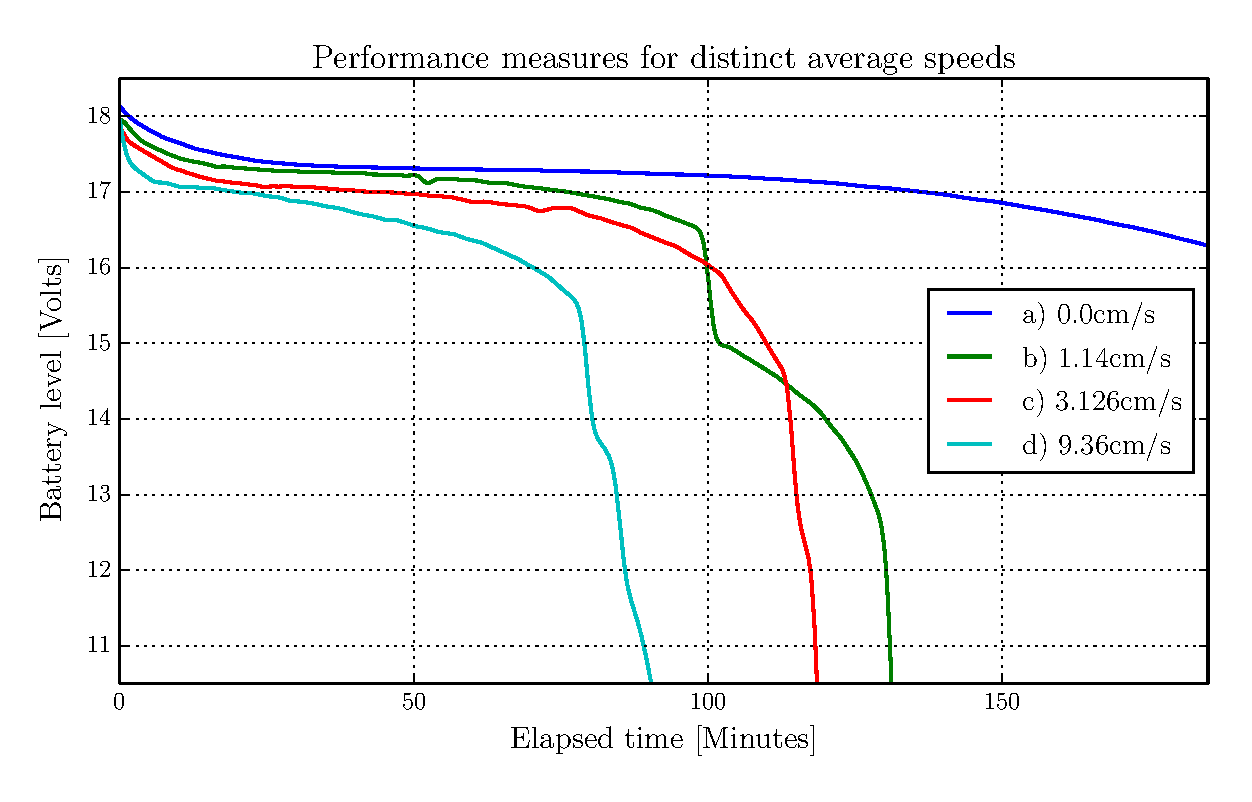
\includegraphics[width=14cm]{images/experiments/battery_performance.eps}}}
\captionFigure{Battery life measurements for distinct average speeds}
{fig:experiments/battery_performance}{
One GNBot powered by two fully-charged 9V 300mAh rechargeable batteries in series configuration was the setup used for this study. A simple obstacle-avoidance routine was used to ensure the continuous motion of the robot.
The cross of curves \emph{b)} and \emph{c)} at $t=100min$ and $t=112min$ shows the variability among the same batch of batteries, and is probably due to differences in charging history.
\emph{Operating time: a) 255min b) 131min c) 119min d) 91min}.
\emph{Distance range estimation: a) 0m b) 90.29m c) 222.26m d) 505.44m}.
}
\end{figure}



The measurements in Figure \ref{fig:experiments/battery_performance} show that servomotors do not have a linear \emph{power/performance} relationship, as they maintain a very high power consumption even at very low speeds. Using this information the search strategy can be adapted to maximize search range. This can be done, for instance, by disabling the motion of the robot when waiting for a sensor measurement to be completed.
The knowledge of various differentiated stages on the battery life is useful information that can be incorporated to trigger a decision-making event during search, to optimize the use of energy resources.
For example, abrupt changes on battery level can trigger a speed change, shutting down high consumption sensors such as the electronic nose, or altering the decision of which robot approaches a given target.
In the case of search strategies based on L\'evy walks, the motion decision extracted from the L\'evy distribution can also be modulated in real time with the battery life estimation.


\lsection{Odor sensing and detection capability}

Apart from bio-inspired energy management, sensing often requires to implement gain control in different sensory modalities to better adapt to variability in each environmental context. Modulation of the temperature of single odor sensors can serve as a virtualization of sensor arrays and it also allows for spatio-temporal encoding which can be needed for more advanced detection and classification tasks. The GNBoard is conveniently provided with the circuitry necessary to achieve this sort of adaptive modulation in odor sensing, and the functionality has been tested to perform as the original \emph{Olus} module (cf. Fig. \ref{fig:introduction/OlusAndTGS2600}).

Whilst odor sensing capability could have been evaluated as a standalone functionality, the multimodal characteristics of robotic search problems make it mandatory to have actual field measurements that demonstrate odor sensing performance. Also, as odor sensing is one of the most characteristic parts of the GNBot design, it is more than convenient to document these features.
Figure \ref{fig:experiments/roomForTests} shows the area utilized for the field odor detection experiments.

\begin{figure}[h!]
\centerline{\mbox{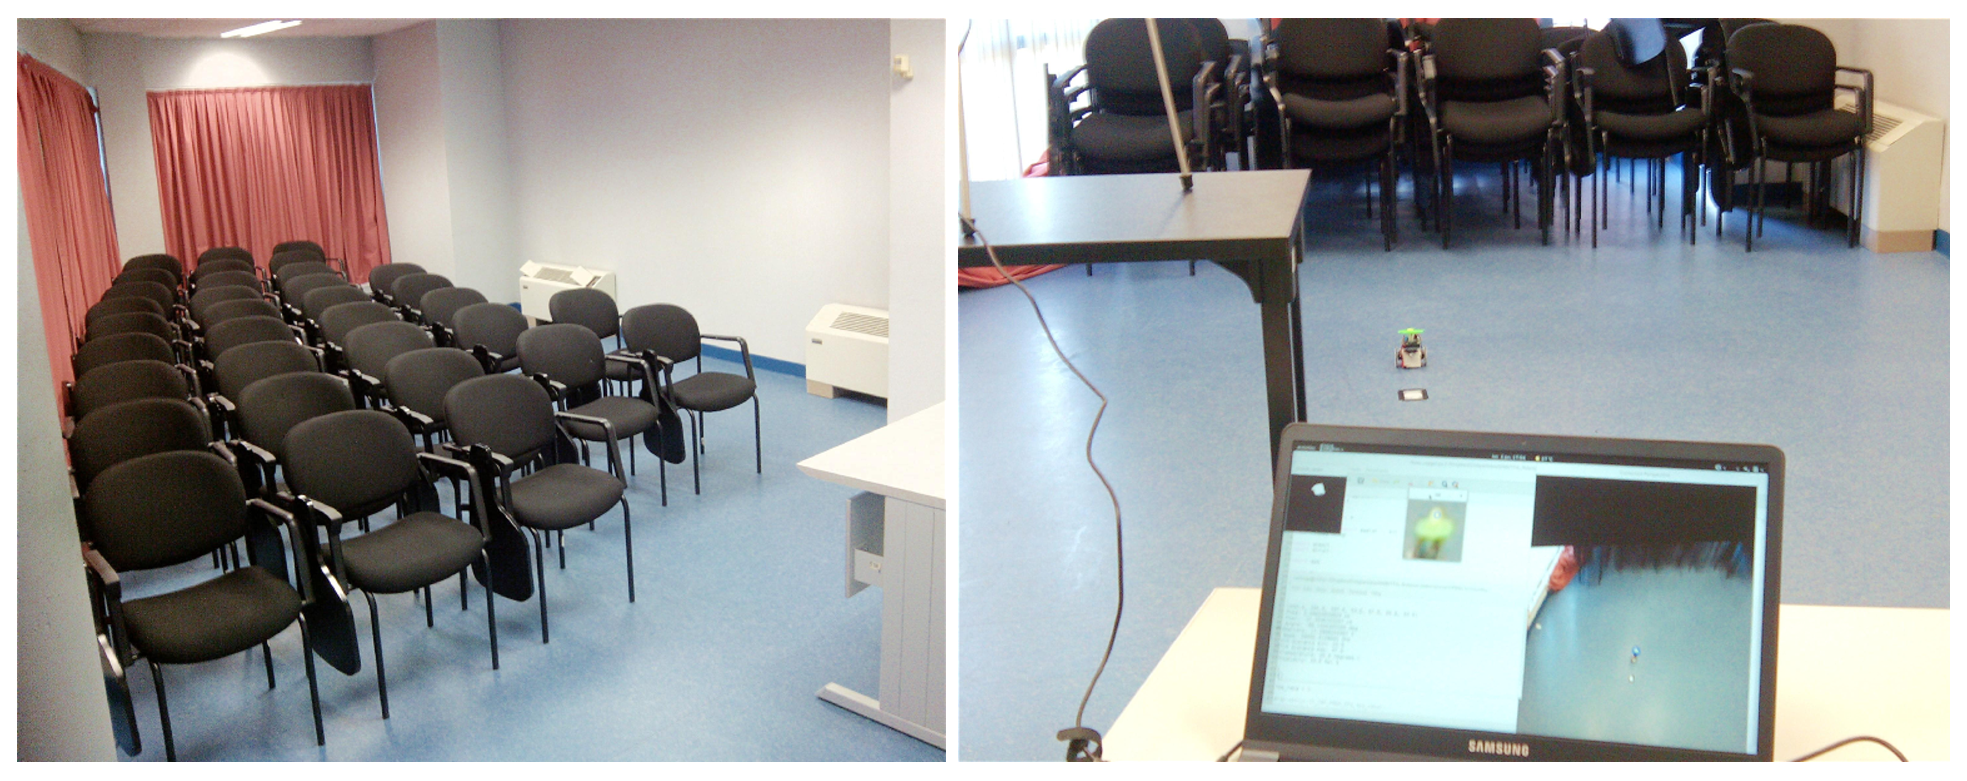
\includegraphics[width=16cm]{images/experiments/roomForTests.eps}}}
\captionFigure{Room used for the tests (left) and an experiment in progress (right)}
{fig:experiments/roomForTests}{
The chairs were moved to the back of the room before each experiment in order to have free space. Also, the air conditioning system was turned off and all windows were closed to minimize air flow. The picture on the right shows the robot approaching an odor source while the computer-vision algorithm tracks the position of the on-board visual marker.
}
\end{figure}


As each search problem can have a different definition of the characteristics of an odor source, the platform validation tests were performed for two different odor source types (shown in Fig. \ref{fig:experiments/GNBot_and_odorSources}). The evaluation of various odorant targets can also serve to demonstrate the flexibility and easy reconfiguration of the sensors in the robot platform.




\begin{figure}[h!]
\centerline{\mbox{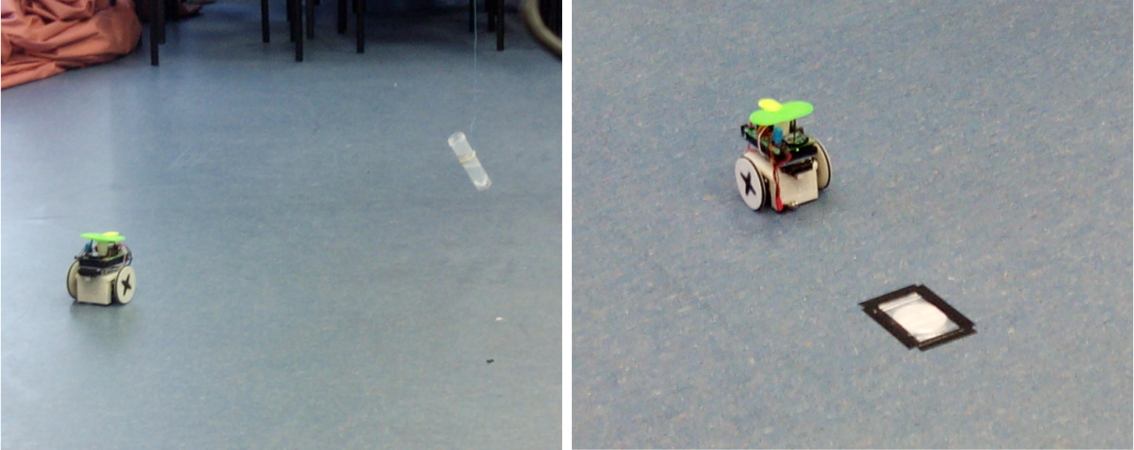
\includegraphics[width=15cm]{images/experiments/GNBot_and_odorSources.eps}}}
\captionFigure{GNBot and different odor sources}
{fig:experiments/GNBot_and_odorSources}{
The odor source on the left is an open tube containing a 50\% solution of ethanol, which is attached to the ceiling with a wire and suspended at 5cm above the robot. The low-profile target odorant on the right is based on a flat cotton pad impregnated with the same ethanol solution, and contained in a plastic bag with a circular aperture ($D=1cm$) from where the odor plume escapes.
Both odor sources were successfully detected by the GNBot, but the one on the right panel produced more repeatable results as the effect is much more local.
}
\end{figure}








\begin{figure}[h!]
\centerline{\mbox{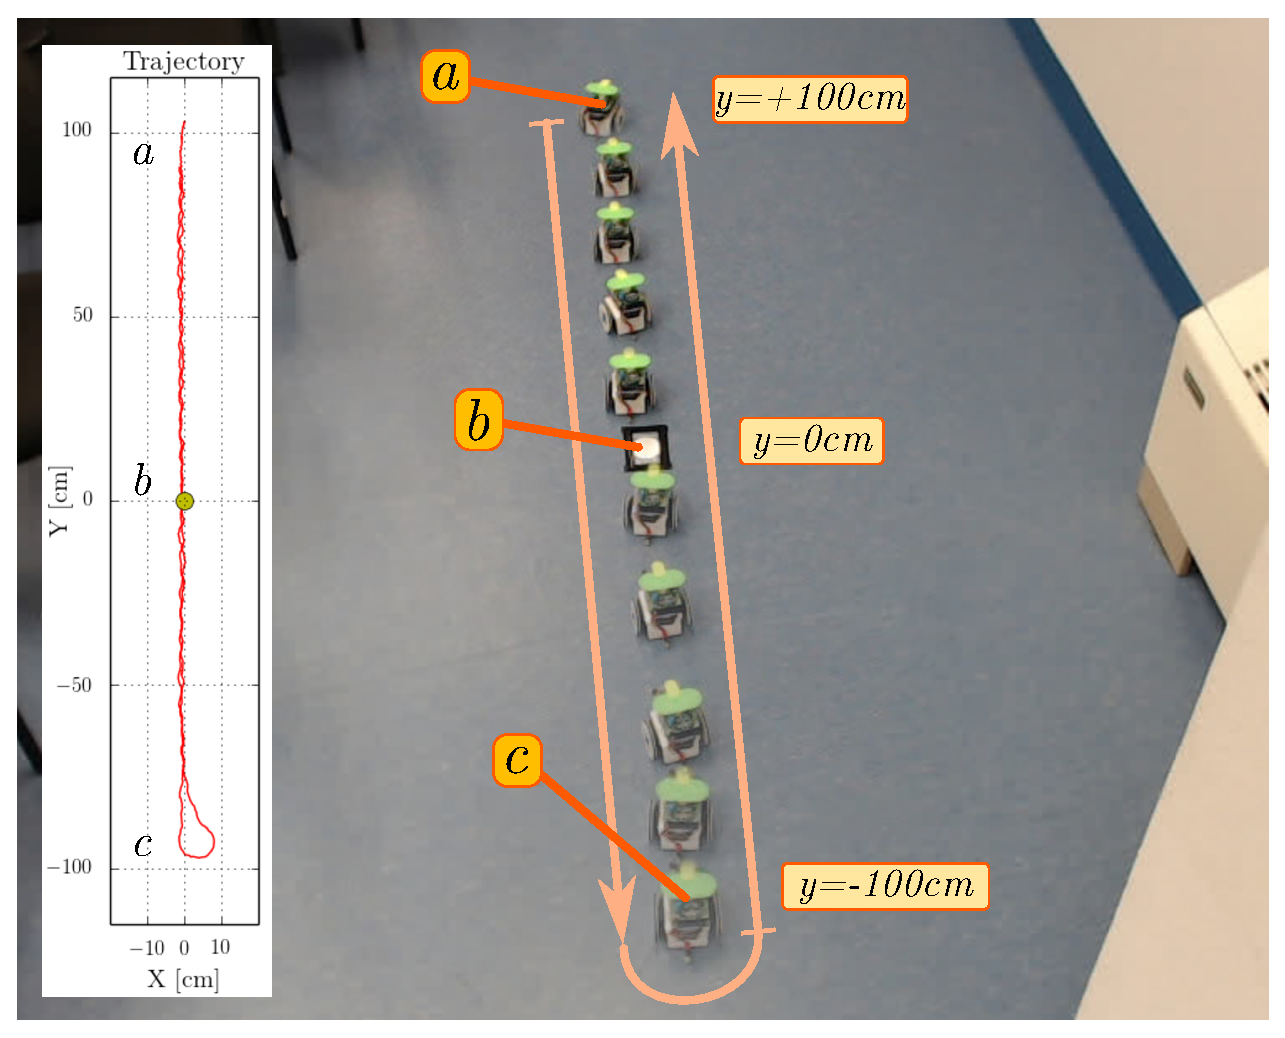
\includegraphics[width=13.5cm]{images/experiments/linearOdorMap.eps}}}
\captionFigure{Closed-loop robot trajectory over an odor source}
{fig:experiments/linearOdorMap}{
The odor source is adhered to the center of the test area \emph{(b)}.
For the target characterization, the robot performs two passes in opposite directions ($a \rightarrow b \rightarrow c$ and $c \rightarrow b \rightarrow a$). The developed navigation software autonomously commands the robot, closing the control loop with the incorporation of feedback from the visual marker tracking algorithm.
The position of the robot and all sensor measurements are logged in the computer in real time ($T=100ms$).
}
\end{figure}



In order to validate the odor sensing functionality, the decision was to perform basic tests to determine the correlation among the variables \emph{distance to an odor source} and \emph{perceived odor intensity}.
For that purpose, the autonomous navigation capacity of the GNBot was used to execute controlled linear approaches to the odor sources. Figure \ref{fig:experiments/linearOdorMap} describes the methodology of the experiment.


\vspace{-0.3cm}

\subsection{Vision-based robot localization system accuracy}

\vspace{-0.3cm}

Figure \ref{fig:experiments/linearOdorMap} can also be used to ilustrate the autonomous positioning capacity of the developed platform. A camera observing the area of the experiment is controlled by the central computer, where a machine-vision algorithm evaluates the position of each robot in the test environment.
The vision-based system has been possible since high resolution cameras have become low-cost and widely available. The precision in the position and angle measurements is better than $\pm 5cm$, which is quite acceptable, specially when compared to the size of the robots ($10$x$10cm$).
This resolution should be enough for most search algorithm implementations. The system is also highly scalable: placing multiple cameras in the ceiling would allow to monitor larger surfaces without too much overhead in cost.



\vspace{-0.3cm}

\subsection{Odor detection results}

\vspace{-0.3cm}

Characterization results for a low-profile odor source are shown in Figure \ref{fig:experiments/odor_sensor_measurements}.
\begin{figure}[h!]
\centerline{\mbox{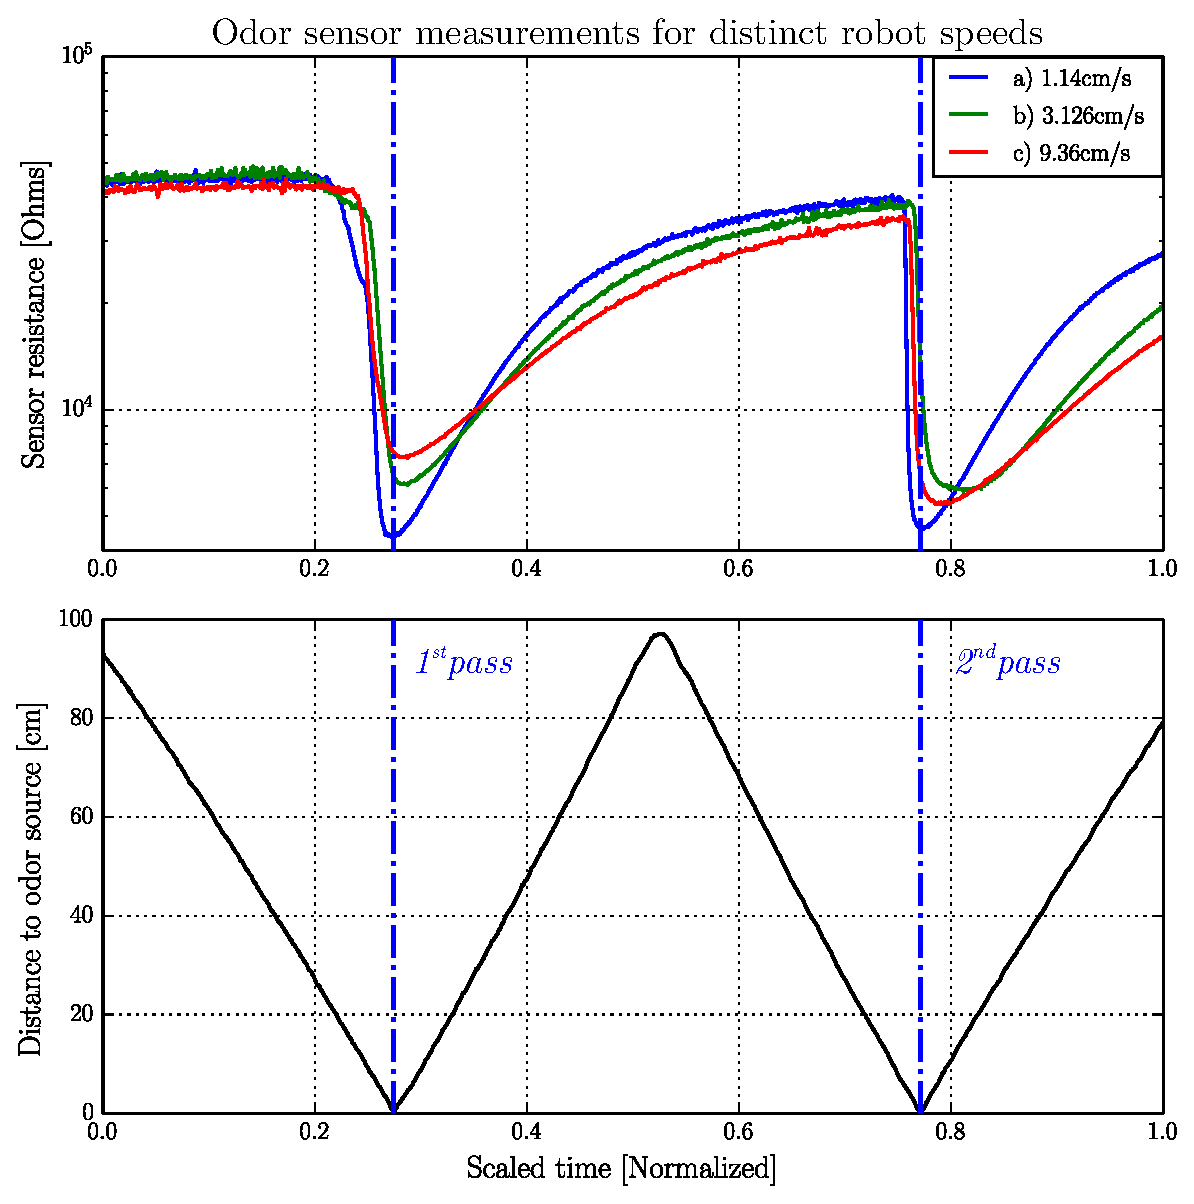
\includegraphics[width=12.5cm]{images/experiments/odor_sensor_measurements.eps}}}
\captionFigure{Odor sensor measurements for distinct robot approximation speeds}
{fig:experiments/odor_sensor_measurements}{
Sensor resistance is shown in the top panel, and the actual euclidean distance to the odorant is represented in the bottom.
For the data generation, the robot performs two passes right over the odor source, as shown in Fig. \ref{fig:experiments/linearOdorMap}.
The TGS-2600 gas sensor mounted on board the GNBot works as a resistance whose value varies in relation with the perceived odor intensity.
A reduction of resistance indicates the detection of a significative amount of odorant molecules in air. That way it is possible to identify the presence of an odor source as a falling edge in the resistance of the odor sensor, or with a simple threshold detector (i.e. $R<10k\Omega$).
The double pass of the robot over the odorant allows to determine the hysteresis in sensibility, which is related to the delay needed for normal operation after the saturation of the sensor.
}
\end{figure}
It can be appreciated that odor detection begins for the three cases at around $20cm$ from the odor source, which is the effective range that could be incorporated in search strategies.
The initial hypothesis was that for higher robot velocities the sensor response would be more abrupt, but the obtained results have shown the opposite effect: resistivity reaches lower values for more reduced speeds.
The updated hypothesis is related with the physical characteristics of the TGS-2600 odor sensor, whose sensitivity to odorant concentrations seems to become intensified for longer exposure periods.
Thus, it would be possible to modulate the localization algorithms to adjust the detection threshold according to the velocity of the robot, in order to maximize sensitivity even at high speeds.




Further odor detection tests are detailed in Figure \ref{fig:experiments/5x5reticularMap}. Even with the uncertainty introduced by the use of a suspended odor source rather than a low-profile one, the detection can be successfully achieved.
\begin{figure}[h!]
\centerline{\mbox{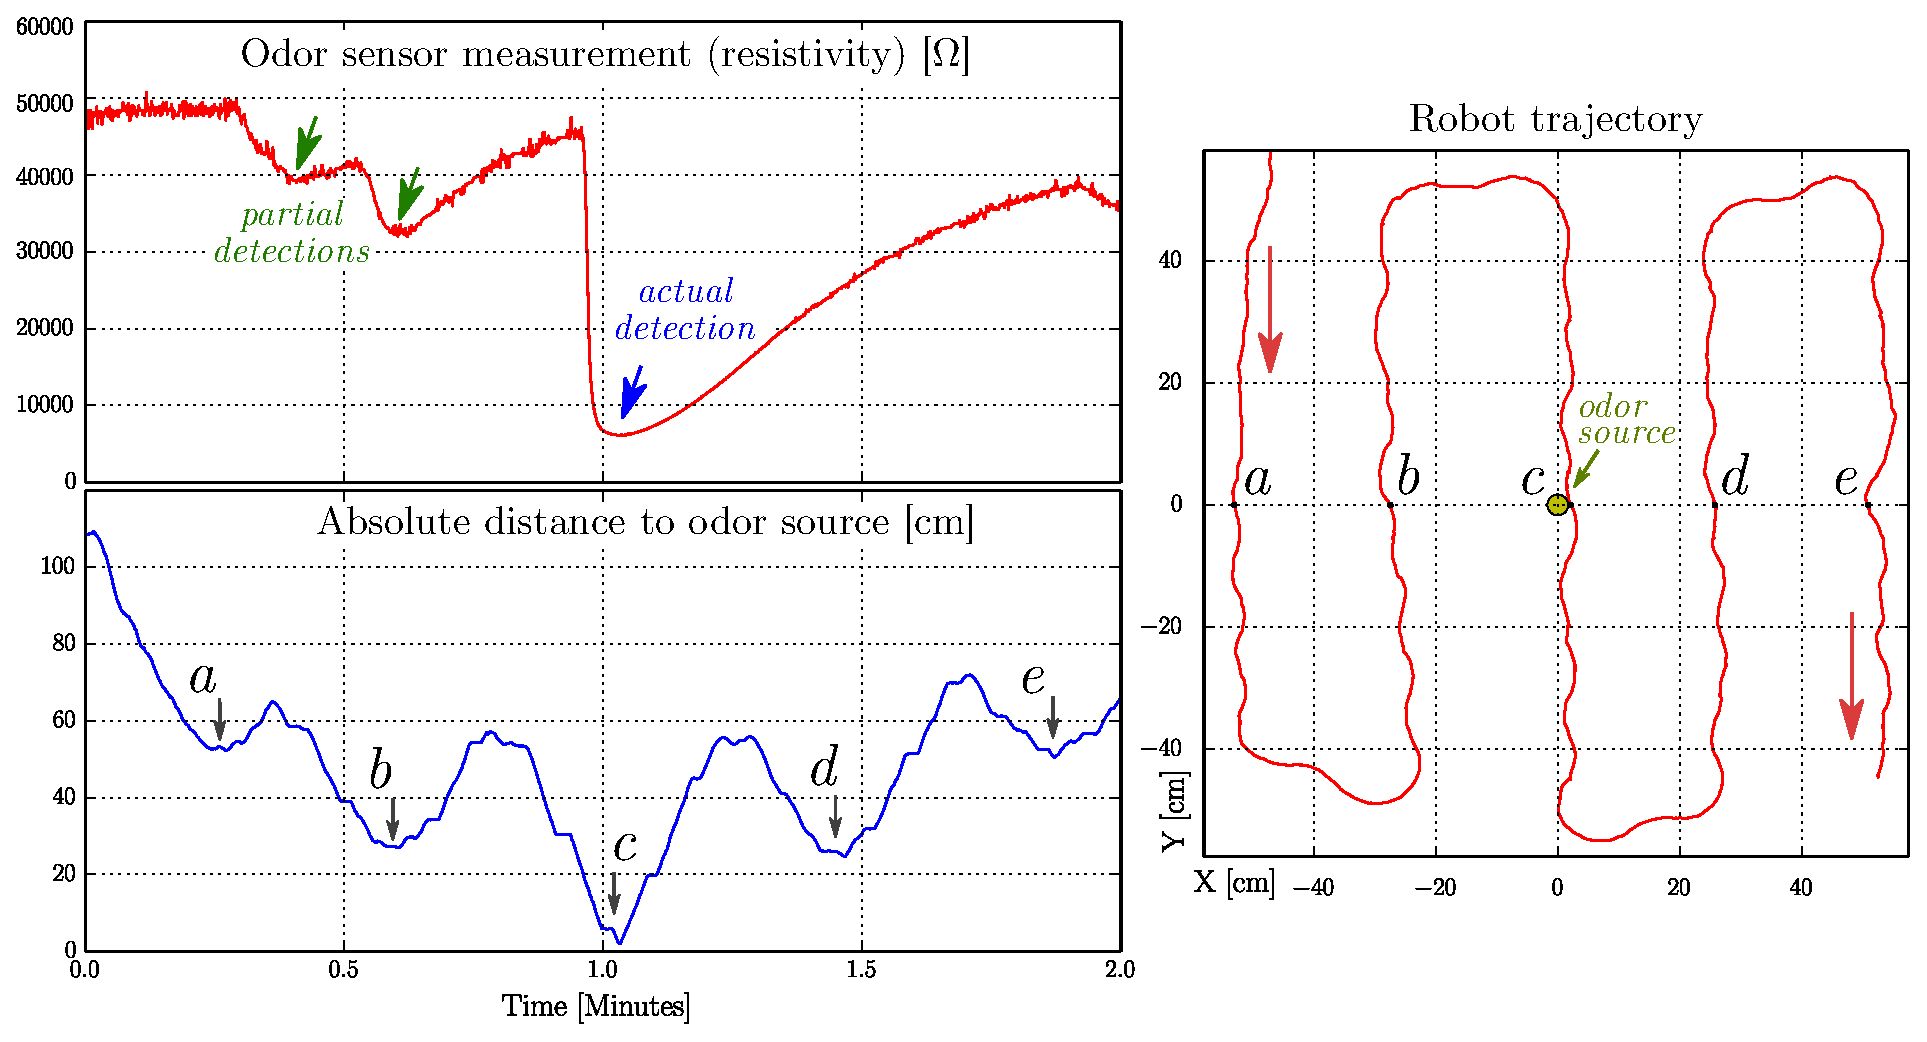
\includegraphics[width=16cm]{images/experiments/5x5reticularMap.eps}}}
\captionFigure{Odor sensor test with a 2-D trajectory}
{fig:experiments/5x5reticularMap}{
For this experiment the navigation algorithm commanded the robot to perform a zig-zag trajectory that combines a set of odor source approximations (see right panel).
The resulting measurements are shown in the left panels: the sensor response (top) and the absolute value of the distance to \emph{c} (bottom).
The suspended odor source in position \emph{c} can be perceived in the measurements even when the robot is near positions \emph{a} and \emph{b} (marked as \emph{``partial detections''}).
Simple threshold detection (i.e. $R<10k\Omega$) applied to the odor sensor response could effectively inform of the presence of the target just before the robot arrival ($t=1min$).
}
\end{figure}




The other factor that can be highlighted from measurements in Figures \ref{fig:experiments/odor_sensor_measurements} and \ref{fig:experiments/5x5reticularMap} is the recovering time -\emph{hysteresis}- of the odor sensor. Whilst the plume detection occurs quite fast, lasting only a few seconds, it can be appreciated that the saturation of the sensor lasts much longer.
For the highest speed result \emph{(c)} in Figure \ref{fig:experiments/odor_sensor_measurements} it is possible to see that in the second pass the sensor has not yet recovered from the previous detection.
This indicates that for an odor search task were multiple odor sources can appear near each other, the monitoring should be performed at slow speeds \emph{(a)} in order to avoid overlaps.



Finally, the rest of multimodal sensors present in the GNBot were also successfully tested: The frontal infra-red distance sensor provides accuracy in the centimeter scale for close-up distances ($10$-$40cm$), and the humidity and temperature sensors provide a resolution of $\pm1\%$ and $\pm0.5\,^{\circ}{\rm C}$ respectively.
The magnetometer module for the electronic compass provided an accuracy of $\pm0.1\,^{\circ}$ after calibration, though magnetic field distortion could be a problem for indoor environments as it is shown in Appendix \ref{Appendix:lightLandmarks}.
Also, wireless communication with the robots via ZigBee did not present any range related limitations and performed as expected from the manufacturer's specification.



\subsection{Easy replication of the GNBot \& four-robot team}

The replicability of the GNBot design was put to test with the creation of four identical robots (shown in Fig. \ref{fig:design/developedPlatform}). Cost was kept very low, at a total of \EUR{600} with an estimated \EUR{150} per robot.
To put the price in perspective, it is important to consider the amount of multimodal sensors present in the robot, as well as the simplistic programming layer with a resilient communication system. The robots also have a long-lasting battery life as it has been shown in \ref{sect:batterylife}.

%\begin{figure}[h!]
%\centerline{\mbox{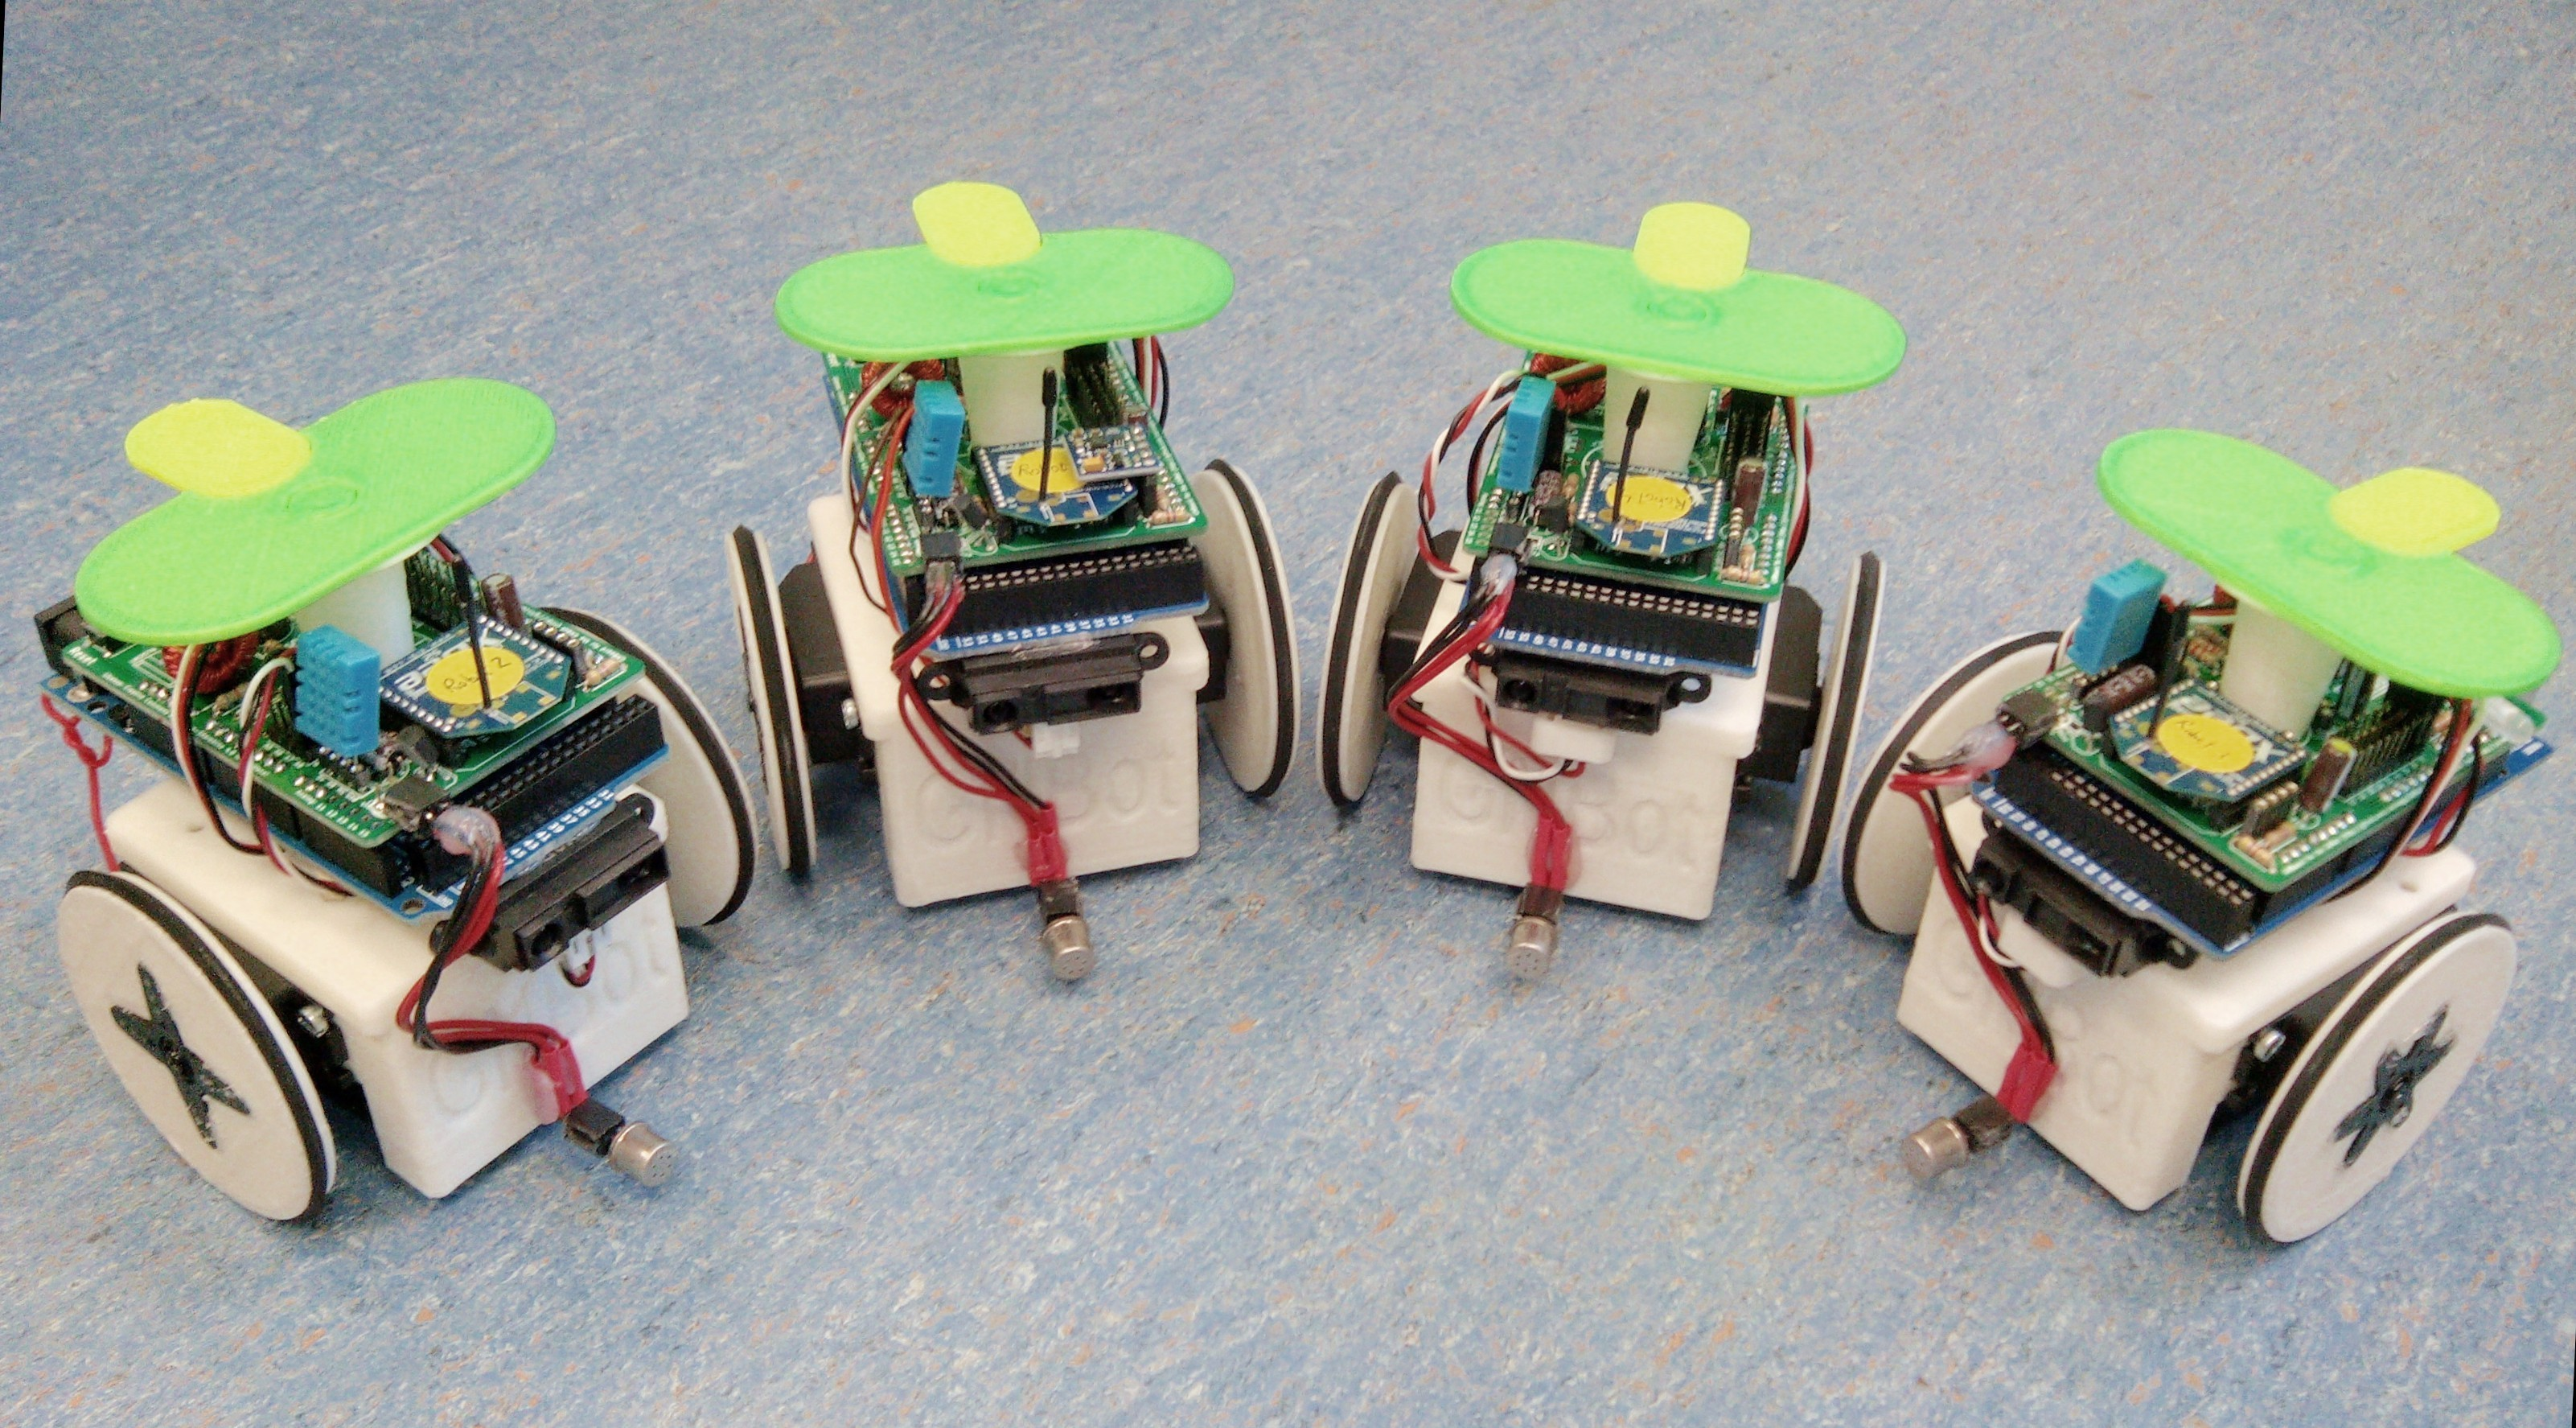
\includegraphics[width=16cm]{images/GNBot_swarm1.jpg}}}
%\captionFigure{Developed robot swarm}
%{fig:GNBot_swarm1}{
%Four identical GNBot robots equipped with a frontal TGS-2600 odor sensor.
%}
%\end{figure}

Apart from robot validation, the next scientific use for these robots
will be the implementation and real-world validation of a bio-inspired collaborative L\'{e}vy strategy developed at \emph{Grupo de Neurocomputaci\'{o}n Biol\'{o}gica} for the search of multiple odor sources in the environment.
Other strategies will be later on tested and their performance compared in a real environment, all thanks to the presence of the GNBot as a standardized robotic platform.

\newpage 

\begin{figure}[h!]
\centerline{\mbox{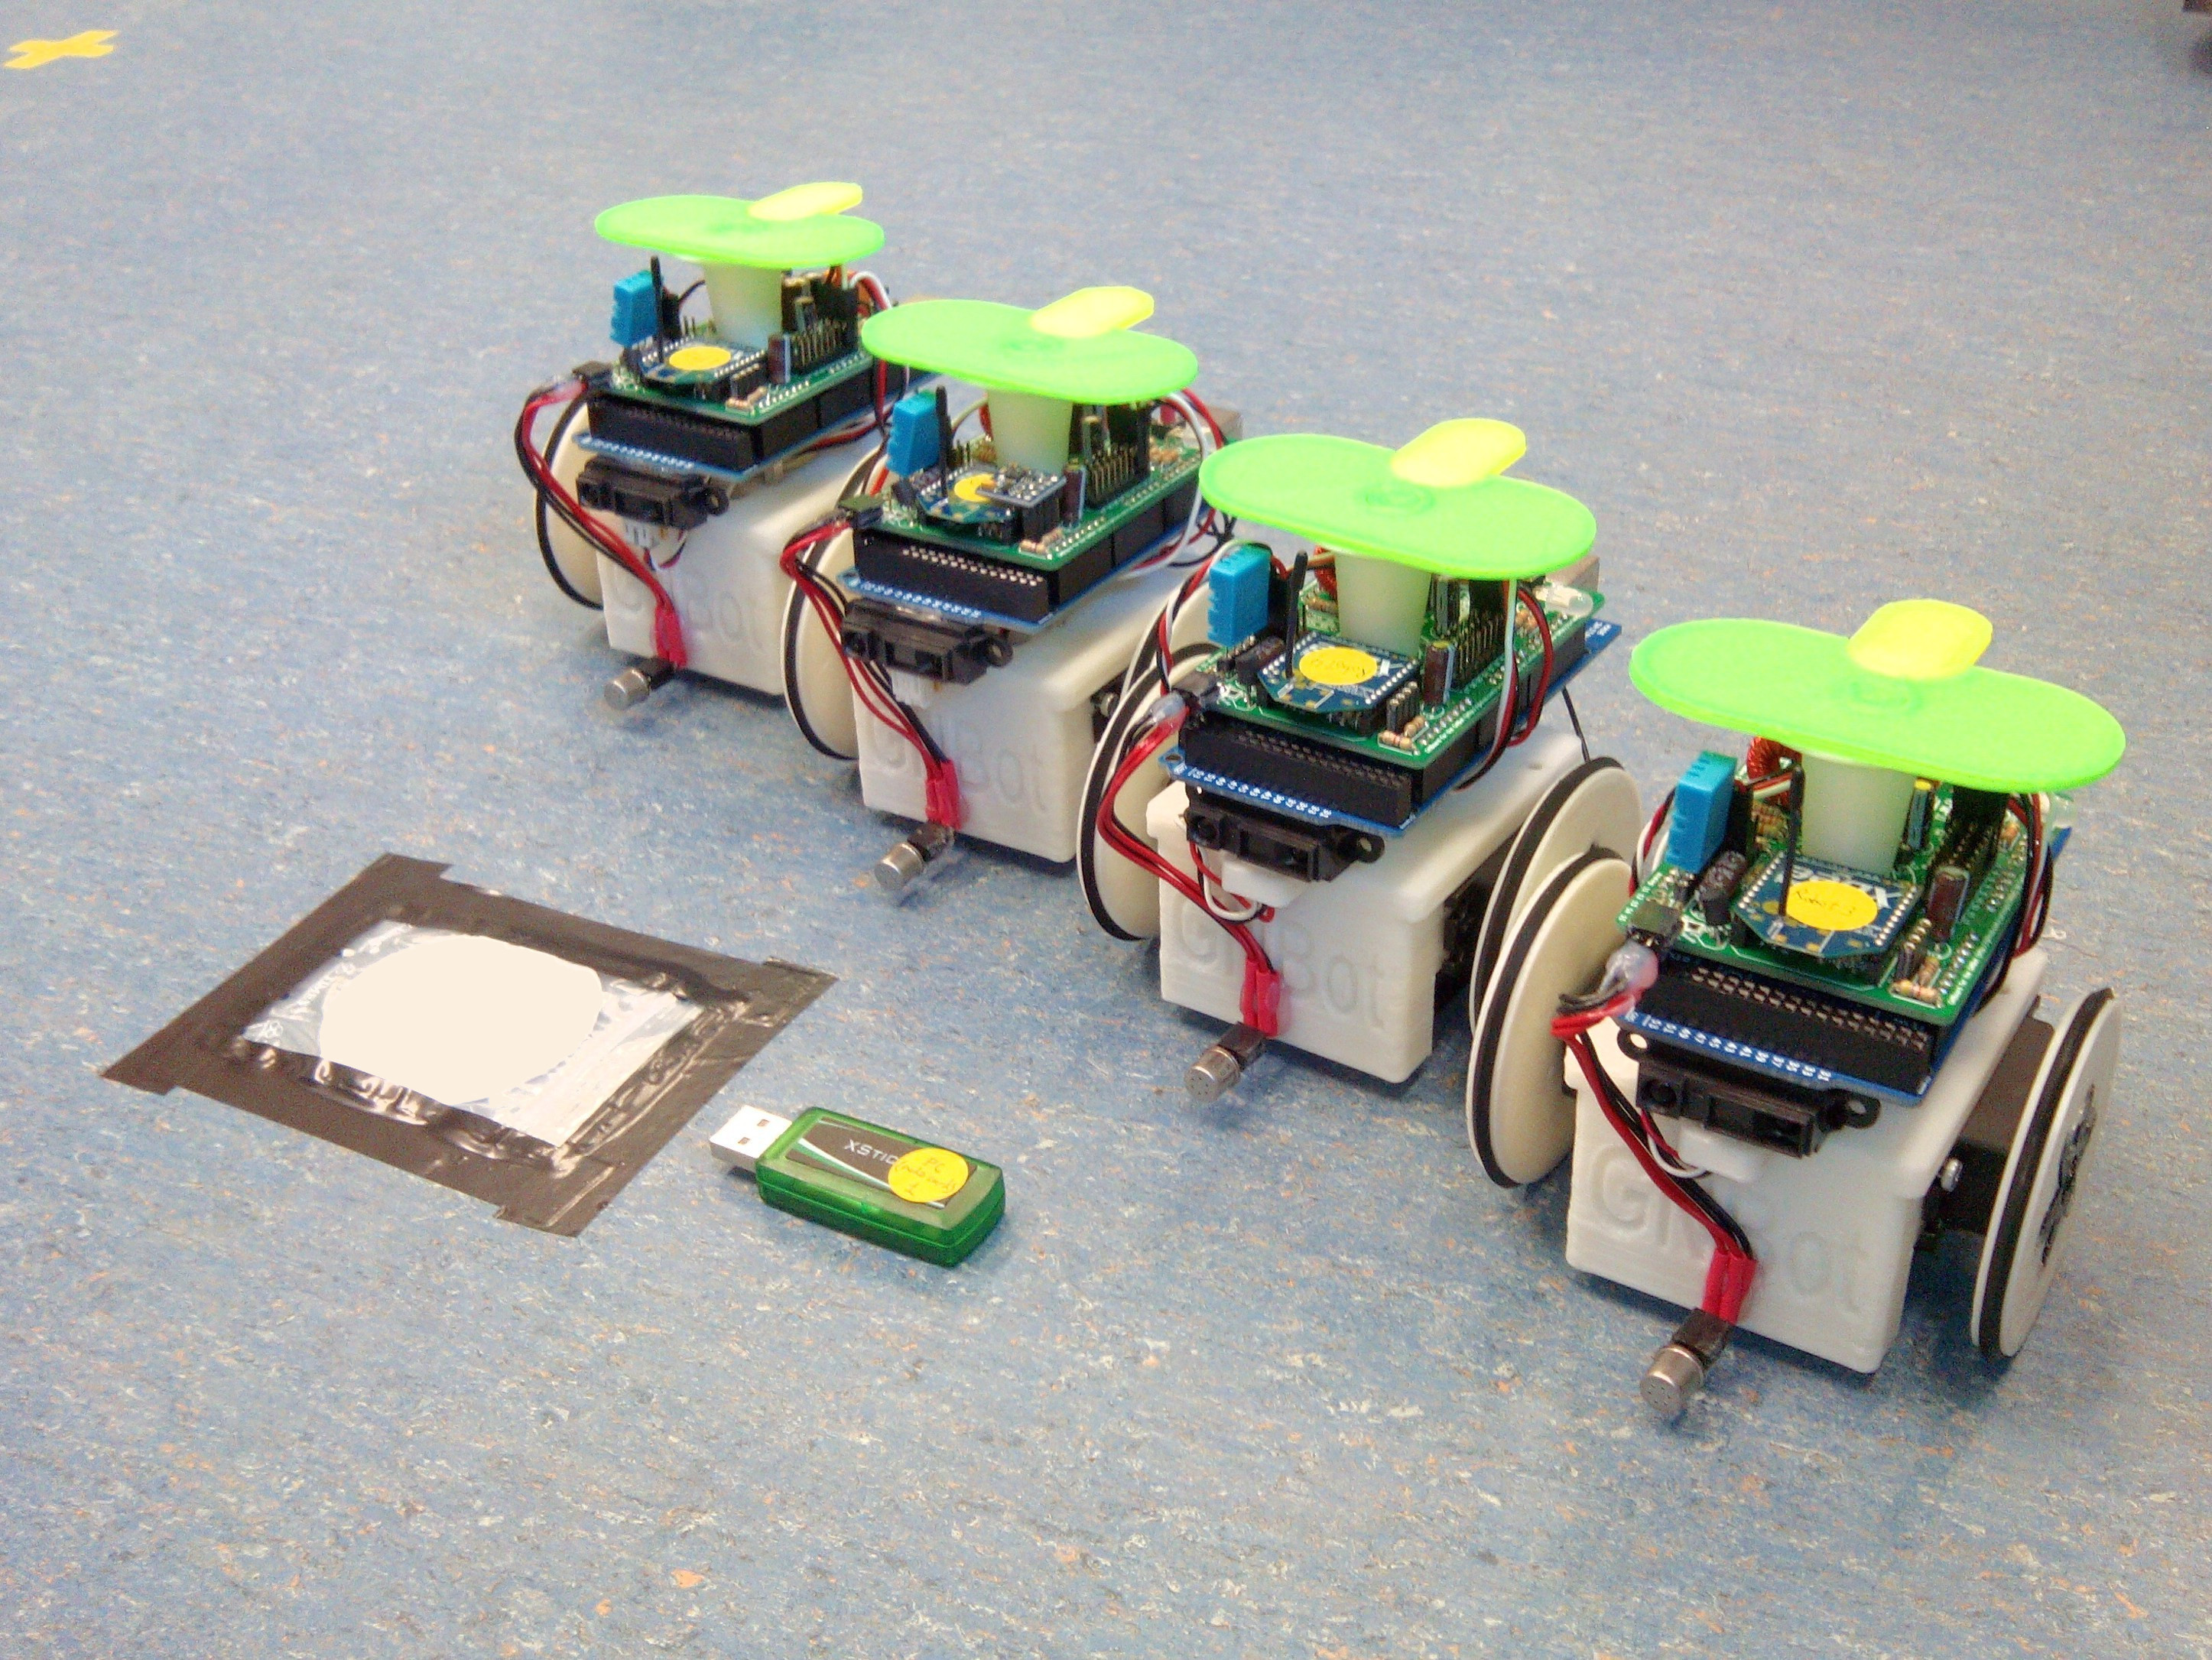
\includegraphics[width=12.5cm]{images/design/developedPlatform.jpg}}}
\captionFigure{Developed robot platform}
{fig:design/developedPlatform}{
The outcome of the project is a swarm of four remotely-controlled robots that have multimodal sensory input (perceiving light, distance, temperature, humidity and orientation with an electronic compass) and are capable of detecting odor sources such as the low-profile target shown on the left.
These robots are also energy efficient, open-source and easy to expand.
The developed system will allow the implementation of a great variety of cooperative search strategies, including those that use range information from each sensor modality with a characterization of the uncertainty of odor sources, and also the ones that use classical heuristic or brute-force approaches for search. Most importantly, the standardization of the platform could finally provide a fair base of comparison for evaluating differences in efficiency among these odor search strategies.
}\end{figure}


\newpage \thispagestyle{empty} % Página vacía

